\documentclass[10pt]{beamer}
\usetheme{cambridgeUS}%{Berkeley}%
\mode<presentation>
%\usepackage{beamerthemesplit}
\usepackage{amsmath,amssymb,latexsym,epsfig,graphics}
\linespread{2}

\title{Approximations to the distributions of quadratic forms in normal variables}
\author{Sha Yu}
\institute[UNCC]
{
	University of North Carolina at Charlotte
}
	
\begin{document}
	
	\frame{\titlepage}

\begin{frame}
\frametitle{Overview}
	\begin{enumerate}
		\item Introduction
		\item Five approximation approaches
		\item Numerical examples simulation
		\item Comparisons and discussion
		\item Conclusion
	\end{enumerate}
\end{frame}	

\section*{Introduction}
	
\begin{frame}
	\begin{itemize}
	\item Consider the quadratic form $Q(X)=X'AX$
	\item X follows an n-dimensional multivariate normal distribution with mean vector $\mu_x$ and non-singular variance matrix $\Sigma$	
	\item A is an $n \times n$ symmetric and non-negative definite matrix
	\item A problem of interest is to evaluate the probability 
	\begin{align}
	Pr(Q(X)>q
	\end{align}
	\end{itemize}
\end{frame}
	
\begin{frame}
	\begin{itemize}
		\item The quadratic form Q can be expressed as a weighted sum of independent chi-square random variables
		\[Q=X'AX=Y'{\Lambda}Y=\sum_{r=1}^m\lambda_r\chi_{hr}^2(\delta_r)\]
		\begin{itemize}
			\item P be a $n \times n$ orthonormal matrix which converts $B={\Sigma}^{1/2}A{\Sigma}^{1/2}$ to the diagnoal form $\Lambda=diag(\lambda_1,...,\lambda_n)=PBP'$, where $\lambda_1\ge...\lambda_n\ge0$
			\item$Y=P\Sigma^{-1/2}X$ is normally distributed with mean $P\Sigma^{-1/2}\mu_x$ and variance In	
			\item $m=rank(A)$; $h_r=1$; $\delta_r=\mu_{yr}^2$, and $\mu_{yr}$ is the ith component of $\mu_y$
		\end{itemize}
	\end{itemize}
\end{frame}

\begin{frame}
	\begin{itemize}
			\item Why do we study the distribution of quadratic forms?
			\item Estimating the tail probability of Q(x) arises in many statistical applications.	
		\begin{enumerate}
				\item The power analysis of a test procedure if the (asymptotic) distribution test statistic(e.g., Peason's chi-square statistic) takes the form Q(X).
				\item Chernoff-Lehmann test statistic for goodness-of-fit to a fixed distribution converges to quadratic forms under the null hypothese.
				\item In time series analysis, Box-Pierece-Ljung portmanteau test statistic for lack of fit in ARMA models converges in distribution to a weighted sum of non-central chi-square random variables under local alternatives.
			\end{enumerate}
	\end{itemize}	
\end{frame}

\begin{frame}
	\begin{itemize}
			\item Why do we approximate the distribution of quadratic forms?
			\item Computing (1) is usually not straightforward except in some special cases. 
			e.g., when $A\Sigma$ is idempotent matrix of rank p,then \[  Q(X)\sim \chi_{p,
				\lambda}^2\]
			\\
			where $\lambda={{\mu_x}'}A\mu_x$
			\item Otherwise, there is no closed analytic expressions.
	\end{itemize}
\end{frame}

\section{Five approximation approaches}
\begin{frame}
	\begin{itemize}
		\item Many methods have been proposed to compute (1).
		\begin{enumerate}
			\item Imhof's approximation 
			\item Farebrother's approximation 
			\item Pearson three-moment central $\chi^2$ approximation 
			\item Liu-Tang-Zhang's four-moment non-central $\chi^2$ approximation
			\item Kuonen's saddle point approximation 
		\end{enumerate}
	\end{itemize}
\end{frame}

\begin{frame}
	\begin{itemize}
		\item Imhof's approximation
		\item Imhof proposed this method relying on numerical inversion of the characteristic function of $Q(x)=\sum_{r=1}^m\lambda_r\chi_{hr}^2(\delta_r)$	
		\[F(x)=\frac{1}{2}-\frac{1}{\pi}\int_{0}^{\infty}t^{-1}g(e^{-itx}\phi(t))dt\]\\
		where $g(z)$ denots the imaginary part of z;\\
		$\phi(t)$ is the characteristic function of t
		\[\phi(t)=\sum_{r=1}^m(1-2i\lambda_rt)^{-\frac{h_r}{2}}exp(i\sum_{r=1}^m\frac{\delta_r^2\lambda_rt}{1-2i\lambda_rt})\]
	\end{itemize}
\end{frame}

\begin{frame}
	\begin{itemize}
		\item After the substitution $2t=u$ is made, we have
		\begin{align}
	Pr(Q(X)>q\approx\frac{1}{2}+\frac{1}{\pi}\int_{0}^{\infty}\frac{\sin\theta(u)}{u\rho(u)}du 
	    \end{align}
	\begin{small}\\		
	where \[\theta(u)=\frac{1}{2}\sum_{r=1}^m[h_r\arctan(\lambda_ru)+\delta_r^2\lambda_ru(1+\lambda_r^2u^2)^{-1}]-\frac{1}{2}qu\]
	\[\rho(u)=\prod_{r=1}^m(1+\lambda_r^2u^2)^{\frac{h_r}{4}}exp(\frac{\sum_{r=1}^m(\delta_r\lambda_ru)^2}{2(1+\lambda_r^2u^2)})\]
	\end{small}
	\item Hard to compute but can be accurate by bonding the approximation error.
	\item $\lambda_r, h_r  and  \delta_r$ must be determinated explicitly. 
	\item However, it is very time-consuming and challenging to convert quadratic forms into weighted sums of chi-square if A is complex and high dimensional.
	\end{itemize}
\end{frame}

\begin{frame}
	\begin{itemize}
	\item Farebrother's approach
	\item Farebrother based on the results of Ruben (1962) exploit that (1) can be written as an infinite series of central chi-square distributions.
	\begin{align}
	Pr(Q(X)>q)=\sum_{k=0}^\infty c_k Pr(\chi_{2k+\tilde{h}}^2 >\frac{t}{\beta})  
	\end{align}\\
	For any $0< \beta <min(\lambda_1,...\lambda_m)$, where $\tilde{h}=\sum_{r=1}^mh_r$, $\gamma_r=1-\beta/\lambda_r$\\
	$g_k=[\sum_{r=1}^mh_r\gamma_r^k+k\sum_{r=1}^m\delta_r\gamma_r^{k-1}(1-\gamma_r)]/2$
	$ c_0=\prod{r=1}^m (\frac{\beta}{\lambda_r})^{\frac{h_r}{2}};exp(-\frac{\sum_{r=1}^m\delta_r}{2})$; $c_k=k^{-1}\sum_{k=o}^{k-r}g_{k-r}c_r$ for $k\geq1$
	\item Share the similar properties with Imhof's approximation
	\end{itemize}	
\end{frame}

\begin{frame}
	\begin{itemize}
		\item Pearson three-moment central $\chi^2$ approximation 
		\item Pearson's method essentially uses the central $\chi^2$ approximation by reqiring the match of the third-order moment.
		\begin{align}
		Pr(Q(X)>q)\approx Pr(\chi_{l^*}^2 >l^*+t^*\sqrt{2l^*})
		\end{align}\\
		where $l^*=1/s_1^2$ is determined so that Q(X) and $\chi_{l^*}^2$ have equal skewness.\\
		$t^*=\frac{t-\mu_Q}{\sigma_Q}$ and skewness of Q(X) is $\beta_1=\sqrt{8}s_1$
		\item This method is easy to compute and no need to convert quadratic forms into the weighted sum of chi-square.
	\end{itemize}
\end{frame}

\begin{frame}
	\begin{itemize}
		\item Liu-Tang-Zhang's four-moment non-central $\chi^2$ approximation
		\begin{align}
		Pr(Q(X)>q)\approx Pr(\chi_l^2(\delta) >t^*\sigma_X+\mu_X))
		\end{align}\\
		where 	$t^*=\frac{t-\mu_Q}{\sigma_Q}$, $\mu_x = l+\delta$, $\sigma_X=\sqrt{2(l+2\delta)}$
		\item THe parameter $\delta$ and l are determined so that the skewness of Q(X) and $\chi_l^2$ are equal and the difference between the kurtosis is minimized.
		\item This approach does not involve inverting a matrix and it has more accuracy than Pearson's approximation.
	\end{itemize}
\end{frame}

\begin{frame}
	\begin{itemize}
		\item How to decide $\delta$ and l ?
		\item skewness of Q(X) is $\beta_1=\frac{\kappa_3}{\kappa_2^{3/2}}=\sqrt{8}s_1$;kurtosis of Q(X) is $\beta_2=\frac{\kappa_4}{\kappa_2^2}=12s_2$\\
		$k_{th}$ cumulant of Q(X) is $\kappa_k=2^{k-1}(k-1)!(\sum_{r=1}^m\lambda_r^kh_r+k \sum_{r=1}^m\lambda_r^k\delta_r)$
		\begin{enumerate}
			\item If $s_1^2 >s-2$\\
			$a=1/(s_1-\sqrt{s_1^2-s_2})$,   $\delta=s_1a^3-a^2$ and $l=a^2-2\delta$
			\item If $s_1^2\leq s_2$\\
			$a=1/s_1$, $\delta=s_1^3-a^2=0$ and $l=1/s_1^2$\\
			In the case, the result is the same as Peason's approximation.
		\end{enumerate}
	\end{itemize}
\end{frame}

\begin{frame}
	\begin{itemize}
		\item Kuonen's saddle point approximation 
		\item By contrast to the Pearson's method, this method use the entire cumulant generating function.
		\begin{align}
		Pr(Q(X)>q)\approx 1-\Phi(w+\frac{1}{w}log(\frac{v}{w}))
		\end{align}\\
		where $w=sign(\hat{\xi})[2(\hat{\xi}q-K(\hat{\xi}))]^{\frac{1}{2}}$,  $v=\hat{\xi}(K^{''}(\hat{\xi}))^{\frac{1}{2}}$\\
		$\hat{\xi}=\hat{\xi}(q)$ is the saddle point which satisfies the equation $K^{'}(\hat{\xi})=q$\\
	    $K(\xi)=-\frac{1}{2}\sum_{r=1}^mh_rlog(1-2\xi\lambda_r)+\sum_{r=1}^{m}\frac{\delta_r\lambda_r\xi}{1-2\xi\lambda_r}$, $\xi< \frac{1}{2}min \lambda_r^{-\frac{1}{2}}$
	    \item This method gives highly accurate approximations.\\
	    $\lambda_1\geq...\geq\lambda_m$ must be determined explicity.
	\end{itemize}
\end{frame}

\section{numerical examples simulation}

\begin{frame}
	\begin{itemize}
		\item We consider five quadratic forms and compute the values of (1) given different values of q. Use Farebrother's method as gold standard.
		\begin{enumerate}
			\item $Q_1=	0.5\chi_1^2(1)+0.4\chi_2^2(0.6)+0.1\chi_1^2(0.8)$	
			\item $Q_2= 0.9\chi_1^2(0.2)+0.1\chi_2^2(10)	$	
			\item $Q_3= 0.1\chi_1^2(0.2)+0.9\chi_2^2(10)	$	
			\item $Q_4= 0.5\chi_1^2(1)+0.4\chi_2^2(0.6)+\sum_{r=1}^{10}0.01\chi_r^2(0.8)$		
			\item $Q_5=\chi_1^1(1.0)+(0.6)^4\chi_1^2(7.0)$\\
			\footnotesize
			If a time series follows a first-order ARMA model with parameter $\alpha$, the Box-Pirece-Ljung test statistic asymptotic follows $\chi_{m-1}^2+\alpha^{2m}\chi_1^2$.\\
			We set $m=2$, $\alpha=0.6$.
		\end{enumerate}
		\end{itemize}
\end{frame}

\begin{frame}
	\begin{itemize}
	\item R demo
	\item Package ‘CompQuadForm’ (2015) by P.Lafaye
	\begin{itemize}
	\item $imhof(q, \lambda, h, \delta ,epsabs = 10^{-6}, epsrel = 10^{-6})$
	\item $farebrother(q, \lambda, h, \delta ,epsabs = 10^{-6}, eps = 10^{-6})$
	\item $liu(q, \lambda, h)$
    \end{itemize}
    \end{itemize}
\end{frame}

\begin{frame}
	\begin{itemize}
		\item R demo of Pearson's approximation
	\end{itemize}
	\graphicspath{{C:/Users/riyi/Desktop/yusha/fall2015-sha/STAT-5123/project}}
	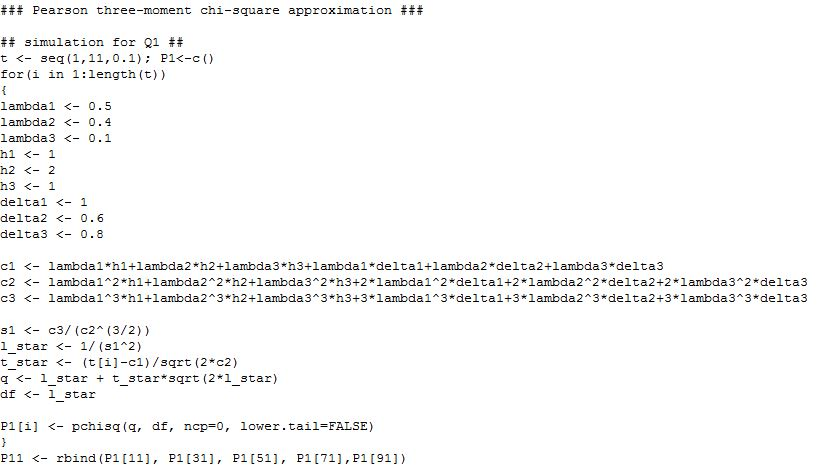
\includegraphics[ scale=.5 ]{Pearson}
\end{frame}

\begin{frame}
	\begin{itemize}
		\item R demo of Kuonen's saddle point approximation
	\end{itemize}
	\graphicspath{{C:/Users/riyi/Desktop/yusha/fall2015-sha/STAT-5123/project}}
	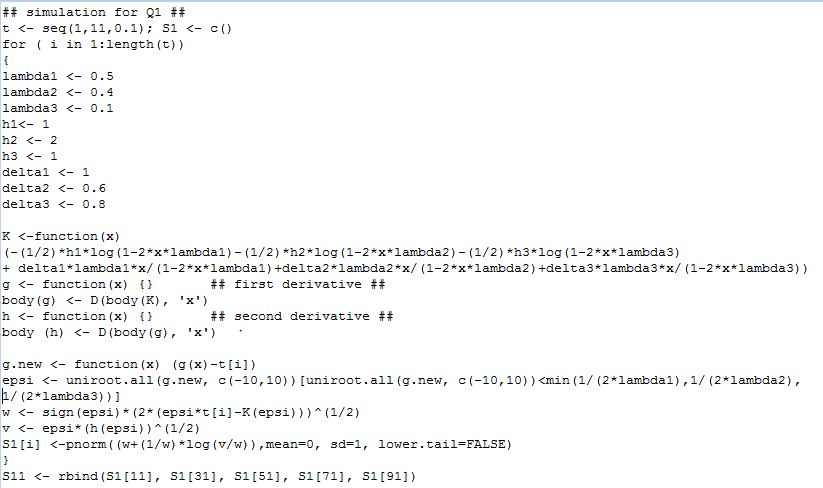
\includegraphics[ scale=.5 ]{Saddle}
\end{frame}

\section{Comparisons and discussion}

\begin{frame}
	\begin{itemize}
		\item R output
	\end{itemize}
	\graphicspath{{C:/Users/riyi/Desktop/yusha/fall2015-sha/STAT-5123/project}}
	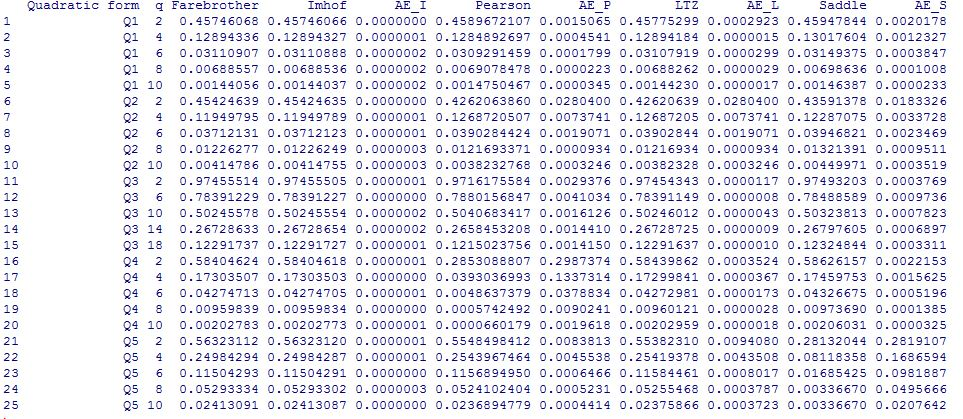
\includegraphics[ scale=.45 ]{table1}
\end{frame}

\begin{frame}
	\begin{itemize}
		\item R output
	\end{itemize}
	\graphicspath{{C:/Users/riyi/Desktop/yusha/fall2015-sha/STAT-5123/project}}
	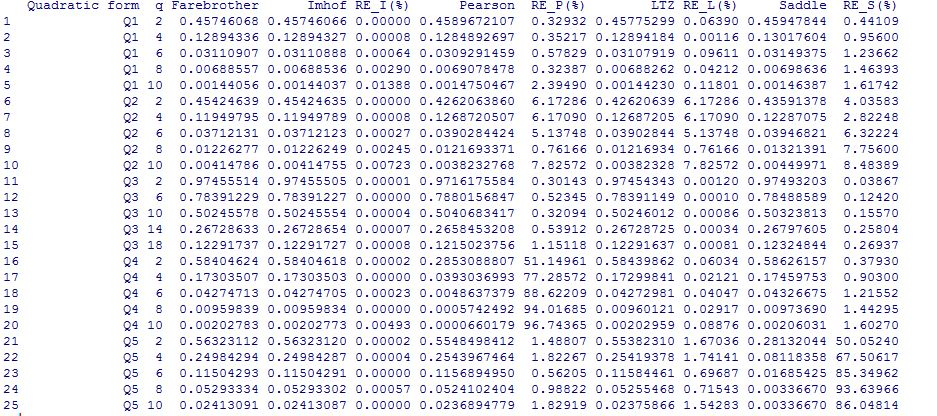
\includegraphics[ scale=.45 ]{table2}
\end{frame}

\begin{frame}
	\begin{itemize}
	\item Compare $Q_1$ and $Q_4$\\	
		\scriptsize
		$Q_1=	0.5\chi_1^2(1)+0.4\chi_2^2(0.6)+0.1\chi_1^2(0.8)$   (red dots)\\
		$Q_4= 0.5\chi_1^2(1)+0.4\chi_2^2(0.6)+\sum_{r=1}^{10}0.01\chi_r^2(0.8)$    (blue dots)	
	\graphicspath{{C:/Users/riyi/Desktop/yusha/fall2015-sha/STAT-5123/project}}
	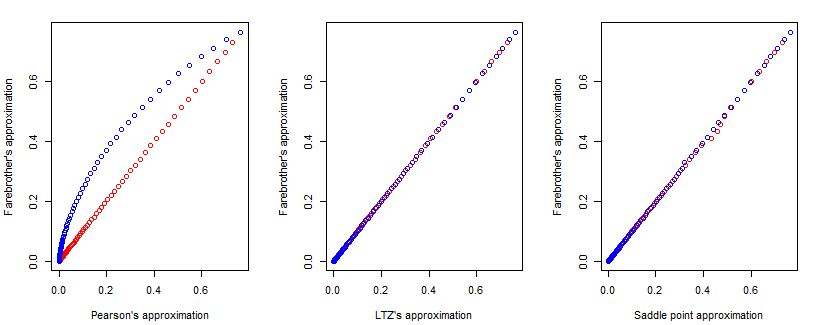
\includegraphics[ scale=0.4 ]{Q1&Q4}
	\footnotesize
	\item Pearson's approximation performs poorly when the number of terms of chi-square increases.\\
	\item The number of terms of chi-square does not affact the accuracy of LTZ's method and Saddle point method.
		\end{itemize}
\end{frame}

\begin{frame}
	\begin{itemize} 
		\item Compare $ Q_2$ and $Q_3$\\	
		\scriptsize
		$Q_2= 0.9\chi_1^2(0.2)+0.1\chi_2^2(10)	$   (red dots)\\
     	$Q_3= 0.1\chi_1^2(0.2)+0.9\chi_2^2(10)	$    (blue dots)	
		\graphicspath{{C:/Users/riyi/Desktop/yusha/fall2015-sha/STAT-5123/project}}
		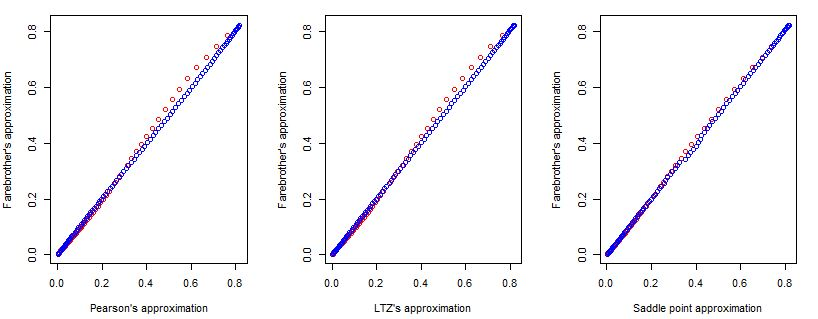
\includegraphics[ scale=0.4 ]{Q2&Q3}
		\small
		\item Pearson's approximation performs better if the chi-square term with large non-centralility parameter has large weight.\\
		\item Weight of the con-central chi-square term does not affact the accuracy of saddle point approximation.
	\end{itemize}
\end{frame}

\begin{frame}
	\begin{itemize} 
		\item What about Q5?\\	
		\scriptsize
		$Q_5=\chi_1^1(1.0)+(0.6)^4\chi_1^2(7.0)$  \\
		Pearson-red dots,  LTZ-blue dots; Saddle point-green dots\\
		\graphicspath{{C:/Users/riyi/Desktop/yusha/fall2015-sha/STAT-5123/project}}
		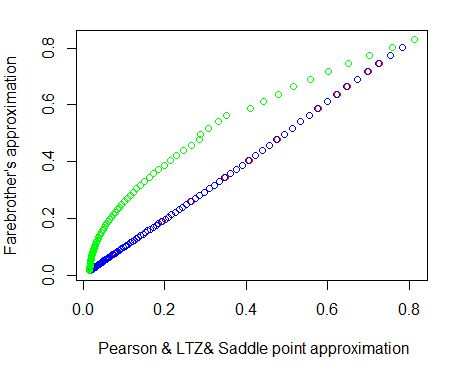
\includegraphics[ scale=0.45 ]{Q5}
		\small
		\item Saddle point approximation performs poorly for Q5.
		\\
		\item Both of LTZ's approximation and Pearson's approximation have high accuracy.
	\end{itemize}
\end{frame}

\section{Conclusion}

\begin{frame}
	\begin{itemize}
		\item Conclusion
		\small
		\begin{enumerate}
		\item Farebrother's method and Imhof's method differ very little.
		\item Pearson's method performs better when the chi-square term with large non-centrality parameter has large weight. It is not appliable when the number of chi-square terms is large.
       \item LTZ's method perfoms much better compared to Pearson's method and it is the most accuracy except the Imhof's method. This method show great advantage if A is complex and high dimensional and thus has great realistic meaning.
       \item Saddle point also has high accuracy but it can not be applied if the sum of coefficeints of chi-square terms is not 1.(Box-Pierce-Ljung statistic)
    \end{enumerate}
\end{itemize}
	
\end{frame}

\end{document}